\subsection{Autonomous Edge Clouds}

%% Edge computing and edge cloud
In edge computing, computing resources are placed at locations close
to the users or data, so as to reduce latencies or to store sensitive
data on premise~\cite{Lopez-2015}.
A possible future direction of edge computing is distributed cloud
computing that utilizes diverse and geographically scattered computing
resources at the edge, and make them act as part of the cloud.

%% edge: from specific purpose to general purpose
Currently, most edge devices are resource-limited, and thus, designed
and used for specific purposes.
However, computing resources could be abundant in the future environment,
if it becomes easier to utilize available computing resources.
Furthermore, we might be able to exploit idle computing resources at
home for a cloud, similar to the way in-house solar power systems are
connected to an electrical grid.
Once there are enough edge resources, they do not need to be
micromanaged and can be used for general purposes.

%% microservice is a driving factor
A driving factor for exploiting available computing resources for cloud
services is the shift to microservices~\cite{nadareishvili2016microservice}
and serverless computing~\cite{Shafiei-2022},
in which a cloud service is composed of a collection of loosely-coupled
lightweight services.
Each microservice is ephemeral and short-lived, and can be executed
in a stateless container,
which enables flexible and efficient use of underlying cloud
resources including smaller edge resources.
%The concept has something in common with early packet switching so
%that it might open up new possibilities to apply packet switching
%techniques to handling microservice jobs.

%% central control to autonomous management
In such an edge cloud, local requests should be handled by local edge
nodes, without being instructed by the central controller.
Thus, cloud management also needs to change from the current central
control to a distributed autonomous model, which requires a
fundamental change to the cloud management model.

\subsection{Cloud Morphing Vision}

\begin{figure}[tb]
  \begin{center}
    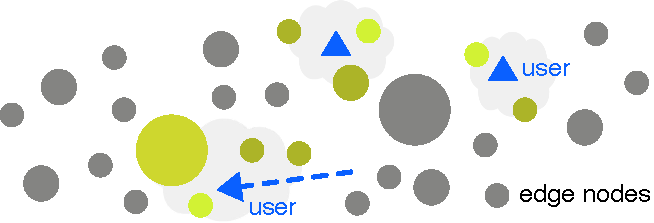
\includegraphics[width=0.8\columnwidth]{morphing-concept.pdf}
    \vspace{-2.0ex}
    \caption{Cloud morphing concept: the shape of a cloud follows the
      usage pattern}
    \Description{Clouds dynamically change their shapes.}
    \label{fig:concept}
  \end{center}
\end{figure}

{\em Cloud Morphing} is our vision for edge clouds in the future.
By dynamically allocating microservices over distributed
heterogeneous resources, a cloud service instance emerges at the best
location and, as the usage pattern changes, the service instance also
transforms the locations of the resources and their connections
(Figure \ref{fig:concept}).

Microservice jobs are assigned to efficiently use required resources
such as computing, communication with the user, access to
database, and other factors.
For examples, an interactive task will follow the user when the user
moves, while a data-intensive task will stay close to the data
regardless of the user location.
Edge computing is automatically formed by allocating resources close to
the users.
Moreover, services are inherently fault-tolerant and resilient
against outages or disasters since faulty resources are
automatically evicted from the resource pool.

From the operational perspective, it can be viewed as virtualization
of cloud infrastrcuture.
Currently, cloud system operators manually manage physical servers and
network switches to meet the overall demands.
By decoupling physical resource management from service management,
cloud service operators are liberated from hardware resource management.

Moreover, it is not enough to shift responsibility to operators of the
new lower infrastructure layer. We need a new self-managing
infrastructure layer which does not require human operators.
The physical resource management becomes simpler with a resource pool.
Physical nodes can be easily attached to or detached from the resource pool.
When there is a consistent hotspot, it can be alleviated or solved by
placing new resources close to the hotspot and then attaching them to
the resource pool at a convenient time.

Diverse resources would be owned and managed by different parties.
It requires loose management of resources, as small parties cannot
afford dedicated skilled operators.
The utilization of each resource needs to be easily manipulated,
without affecting the stability of the system.

To realize such systems, it requires various technical advances across
many fields.  Among other things, new autonomous resource management
model is needed for distributed diverse resources,
which is the topic of this paper.
%% energy saving?
We also take energy saving into consideration as it is
essential for future clouds~\cite{Mastelic-2015,masanet2020recalibrating}.

\subsection{Resource Management}

%% resource allocation problems are NP-hard
%% even harder for distributed heterogeneous resources
Resource allocation in distributed clouds is a non-trivial
optimization problem, and it is even harder when distributed
management is assumed.
%% our idea: use congestion pricing mechanism for automatic load management
To this end, we employ dynamic pricing for decentralized resource
allocation which works as backpressure against congestion.
By design, serious congestion never happens in the system as long as
some resources remain available in the resource pool.
It also reserves a sufficient margin essential for the performance of
statistically multiplexing services.
We use pseudo cost for manipulating resource allocation.
Here, pseudo cost is not an actual monetary charge, but it is used to
control resource utilization; it should not be confused with service
fees for customers.
There exists a large body of literature formulating resource allocation
as optimization problems.
In this paper, we use terms and expressions borrowed from optimization
theory. Our goal is, however, not to pursue theoretical optimum
allocations, but to present a practical feedback control model for
distributed resource management.


